\documentclass[11pt,preprint, authoryear]{elsarticle}

\usepackage{lmodern}
%%%% My spacing
\usepackage{setspace}
\setstretch{1.2}
\DeclareMathSizes{12}{14}{10}{10}

% Wrap around which gives all figures included the [H] command, or places it "here". This can be tedious to code in Rmarkdown.
\usepackage{float}
\let\origfigure\figure
\let\endorigfigure\endfigure
\renewenvironment{figure}[1][2] {
    \expandafter\origfigure\expandafter[H]
} {
    \endorigfigure
}

\let\origtable\table
\let\endorigtable\endtable
\renewenvironment{table}[1][2] {
    \expandafter\origtable\expandafter[H]
} {
    \endorigtable
}


\usepackage{ifxetex,ifluatex}
\usepackage{fixltx2e} % provides \textsubscript
\ifnum 0\ifxetex 1\fi\ifluatex 1\fi=0 % if pdftex
  \usepackage[T1]{fontenc}
  \usepackage[utf8]{inputenc}
\else % if luatex or xelatex
  \ifxetex
    \usepackage{mathspec}
    \usepackage{xltxtra,xunicode}
  \else
    \usepackage{fontspec}
  \fi
  \defaultfontfeatures{Mapping=tex-text,Scale=MatchLowercase}
  \newcommand{\euro}{€}
\fi

\usepackage{amssymb, amsmath, amsthm, amsfonts}

\def\bibsection{\section*{References}} %%% Make "References" appear before bibliography


\usepackage[round]{natbib}

\usepackage{longtable}
\usepackage[margin=2.3cm,bottom=2cm,top=2.5cm, includefoot]{geometry}
\usepackage{fancyhdr}
\usepackage[bottom, hang, flushmargin]{footmisc}
\usepackage{graphicx}
\numberwithin{equation}{section}
\numberwithin{figure}{section}
\numberwithin{table}{section}
\setlength{\parindent}{0cm}
\setlength{\parskip}{1.3ex plus 0.5ex minus 0.3ex}
\usepackage{textcomp}
\renewcommand{\headrulewidth}{0.2pt}
\renewcommand{\footrulewidth}{0.3pt}

\usepackage{array}
\newcolumntype{x}[1]{>{\centering\arraybackslash\hspace{0pt}}p{#1}}

%%%%  Remove the "preprint submitted to" part. Don't worry about this either, it just looks better without it:
\makeatletter
\def\ps@pprintTitle{%
  \let\@oddhead\@empty
  \let\@evenhead\@empty
  \let\@oddfoot\@empty
  \let\@evenfoot\@oddfoot
}
\makeatother

 \def\tightlist{} % This allows for subbullets!

\usepackage{hyperref}
\hypersetup{breaklinks=true,
            bookmarks=true,
            colorlinks=true,
            citecolor=blue,
            urlcolor=blue,
            linkcolor=blue,
            pdfborder={0 0 0}}


% The following packages allow huxtable to work:
\usepackage{siunitx}
\usepackage{multirow}
\usepackage{hhline}
\usepackage{calc}
\usepackage{tabularx}
\usepackage{booktabs}
\usepackage{caption}


\newenvironment{columns}[1][]{}{}

\newenvironment{column}[1]{\begin{minipage}{#1}\ignorespaces}{%
\end{minipage}
\ifhmode\unskip\fi
\aftergroup\useignorespacesandallpars}

\def\useignorespacesandallpars#1\ignorespaces\fi{%
#1\fi\ignorespacesandallpars}

\makeatletter
\def\ignorespacesandallpars{%
  \@ifnextchar\par
    {\expandafter\ignorespacesandallpars\@gobble}%
    {}%
}
\makeatother

\newlength{\cslhangindent}
\setlength{\cslhangindent}{1.5em}
\newenvironment{CSLReferences}%
  {\setlength{\parindent}{0pt}%
  \everypar{\setlength{\hangindent}{\cslhangindent}}\ignorespaces}%
  {\par}


\urlstyle{same}  % don't use monospace font for urls
\setlength{\parindent}{0pt}
\setlength{\parskip}{6pt plus 2pt minus 1pt}
\setlength{\emergencystretch}{3em}  % prevent overfull lines
\setcounter{secnumdepth}{5}

%%% Use protect on footnotes to avoid problems with footnotes in titles
\let\rmarkdownfootnote\footnote%
\def\footnote{\protect\rmarkdownfootnote}
\IfFileExists{upquote.sty}{\usepackage{upquote}}{}

%%% Include extra packages specified by user

%%% Hard setting column skips for reports - this ensures greater consistency and control over the length settings in the document.
%% page layout
%% paragraphs
\setlength{\baselineskip}{12pt plus 0pt minus 0pt}
\setlength{\parskip}{12pt plus 0pt minus 0pt}
\setlength{\parindent}{0pt plus 0pt minus 0pt}
%% floats
\setlength{\floatsep}{12pt plus 0 pt minus 0pt}
\setlength{\textfloatsep}{20pt plus 0pt minus 0pt}
\setlength{\intextsep}{14pt plus 0pt minus 0pt}
\setlength{\dbltextfloatsep}{20pt plus 0pt minus 0pt}
\setlength{\dblfloatsep}{14pt plus 0pt minus 0pt}
%% maths
\setlength{\abovedisplayskip}{12pt plus 0pt minus 0pt}
\setlength{\belowdisplayskip}{12pt plus 0pt minus 0pt}
%% lists
\setlength{\topsep}{10pt plus 0pt minus 0pt}
\setlength{\partopsep}{3pt plus 0pt minus 0pt}
\setlength{\itemsep}{5pt plus 0pt minus 0pt}
\setlength{\labelsep}{8mm plus 0mm minus 0mm}
\setlength{\parsep}{\the\parskip}
\setlength{\listparindent}{\the\parindent}
%% verbatim
\setlength{\fboxsep}{5pt plus 0pt minus 0pt}



\begin{document}



\begin{frontmatter}  %

\title{Utilising Machine Learning Algorithms to Classify Those Most Likely to
Lose Their Main Source of Income due to Lockdown - Evidence From
NIDS-CRAM Wave 1}

% Set to FALSE if wanting to remove title (for submission)




\author[Add1]{Johannes Coetsee - 19491050}
\ead{19491050@sun.ac.za - https://github.com/Coetsee}





\address[Add1]{Stellenbosch University}



\vspace{1cm}

\vspace{0.5cm}
\end{frontmatter}



%________________________
% Header and Footers
%%%%%%%%%%%%%%%%%%%%%%%%%%%%%%%%%
\pagestyle{fancy}
\chead{}
\rhead{July 2021 - Data Science 871}
\lfoot{}
\rfoot{\footnotesize Page \thepage}
\lhead{}
%\rfoot{\footnotesize Page \thepage } % "e.g. Page 2"
\cfoot{}

%\setlength\headheight{30pt}
%%%%%%%%%%%%%%%%%%%%%%%%%%%%%%%%%
%________________________

\headsep 35pt % So that header does not go over title




\hypertarget{introduction}{%
\section{\texorpdfstring{Introduction
\label{Introduction}}{Introduction }}\label{introduction}}

The purpose of this paper is to report on the implementation of two
machine-learning (ML) algorithms for a classification-type problem.
South Africa, like most countries, have undergone severe economic
pressures due to the Covid-19 pandemic and the ensuing hard lockdown.
Many individuals and households have reported that they have lost their
primary source of income due to the latter. This study employs two
different tree-based ML algorithms to help identify who was most likely
to lose their primary source of income given a variety of other
variables. These two algorithms are 1) a baseline tuned Random Forest
(RF), and 2) a simple Gradient-Boosted Model (GBM). This report
therefore compares the accuracy of these algorithms in classifying which
households were more likely to lose their main source of income due to
the coronavirus and subsequent lockdown in South Africa in March and
April 2020.\footnote{The template for this report is based on that
  provided by Katzke (\protect\hyperlink{ref-Texevier}{2017}).}

\hypertarget{data}{%
\section{\texorpdfstring{Data \label{Data}}{Data }}\label{data}}

This study utilises the first wave of the National Income Dynamics Study
- Coronavirus Rapid Mobile Survey 2020 (NIDS-CRAM) dataset, a nationally
representative longitudinal household survey conducted over telephone by
the Southern Africa Labour and Development Research Unit (SALDRU) in
April and May 2020. NIDS-CRAM investigates the various social and
economic effects of the national lockdown implemented in March 2020, and
more broadly, the consequences of the global pandemic on the South
African population Ingle \emph{et al.}
(\protect\hyperlink{ref-nids2020}{2020}).\footnote{Data is publicly
  available at \url{https://www.datafirst.uct.ac.za/}.}

For our analysis, however, a subsample of the NIDS-CRAM dataset was
collected. Emphasis was placed on the first wave, as this would be where
the effects of lockdown would be felt most acutely in terms of loss of
income sources. This is preferable as one wants to build a model that
most accurately classifies between the pre-pandemic and post-lockdown
states. The final dataset consists of 21 features, reported in Table
\ref{Features} below, with 7073 observations in total. Table
\ref{Features} also reports the amount of missing values for each
feature, as well as a relevant description.\footnote{In this case, the
  survey answers `Refused', `Don't Know', `Not Applicable' and `Missing'
  are all defined as NAs.} The main feature of interest is `Income
Change' - a binary variable where a value of 1 indicates that the
household has lost their main source of income, whilst 2 indicates that
it has not. The question asked to respondents reads as follows: ``Has
your household lost its main source of income since the lockdown started
on 27th March?''.

\begin{table}
\begin{center}
\begin{tabular}{ |l|c|l| } 
 \hline
 Selected Features & NAs & Description \\ 
 \hline
  Income Change & 168 &  Has household lost main source of income since lockdown \\ 
  Sources Income Decreased & 376 & Did sources of household income decrease during lockdown \\
  Employed & 161 &  Employment Status \\
  Employment Type & 151 & Respondent's main form of work (0 = unemployed) \\
  Sources HH Income & 121 & Sources of household income in February \\
  Children Change & 93 & Change in number of children in house compared to pre-lockdown \\
  Province & 8 & Province currently living in now \\
  Dwelling Type & 6 & Type of dwelling, whether house, informal, traditional or other \\
  Race & 0 & Respondent's given population group \\
  Geo Type & 8 & Geography Type (derived from 2011 census) \\
  HH Income Apr & 2665 & Total household income after tax in April \\
  Moved & 8 & Whether respondent moved to another dwelling for lockdown \\
  Grant & 36 & Whether the respondent receives any kind of government grant \\
  Electricity Access & 2 & Whether dwelling has access to electricity \\
  Water Access & 5 & Whether dwelling has piped or tap water \\
  HH Size & 32 & Number of people resident (Household Size) \\
  Education & 45 & Highest school grade completed \\
  Tertiary & 9 & Has respondent successfully completed some tertiary education \\
  Age & 0 & Respondent's age in years \\
  Age Interval & 0 & Age interval (5 year intervals) \\
  Gender & 0 & Respondent's stated gender \\
  District Council & 8 & Municipal Demarcations Board District Council (from 2011 Census) \\
  \hline
\end{tabular}
\caption{Features}
\label{Features}
\end{center}
\end{table}

\hypertarget{missing-values-and-transformations}{%
\subsection*{Missing Values and
Transformations}\label{missing-values-and-transformations}}
\addcontentsline{toc}{subsection}{Missing Values and Transformations}

It is evident from \ref{Features} that missing values might be a
stumbling block for accurate analysis. In particular, the `HH Income
Apr' variable has a large amount of NAs, most of which are attributed to
the `Don't Know' category on the questionnaire. In other words,
respondents reported that they did not know their exact level of income
for the month of April 2020. In order to avoid losing potentially
valuable information, this study imputes missing values for all features
within the dataset. Furthermore, NAs for the `Employment Type' feature
are replaced by 0's to indicate `unemployed', as this survey question
was only asked to those who were employed. Those who refused to respond
or did not know their main form of work, were indicated as missing and
therefore imputed. Similarly, system NAs for the `Tertiary' feature - a
dummy variable indicating whether an individual completed some form of
tertiary education - was replaced by 0, or `no', as this question was
only asked to those who were eligible. Although not perfect solutions,
these are fair assumptions to make in order to include these potentially
meaningful variables. Additionally, the feature indicating in which
District Council the household is situated was transformed into a matrix
of binary variables so as to accommodate the necessary structure needed
for imputation.\footnote{This is due to the fact that only 53 levels are
  allowed for factored variables using both the \emph{missForest} and
  \emph{randomForest} packages, whereas the District Council variable
  consists of 54 levels.}

Methodologically, a random forest algorithm - trained on the matrix of
observed values in the data - is used to impute missing values. This can
be done using the package \emph{missForest} in R, which follows a
two-step procedure. First, missing values are pre-imputed using simple
median replacement for continuous data types - where the missing value
is replaced with the median value computed on the rest of the observed
data for each continuous feature. For categorical variables, missing
values are replaced by the most frequently occurring non-missing
value.\footnote{This replacement-procedure is also called Strawman
  imputation.} Second, a forest is grown using multivariate splitting,
where the splitting rule is averaged only over non-missing values. Data
is then imputed by regressing each feature on all other features,
thereafter predicting missing values using the fitted forest. This
process is iterated in order to update the initial median-replaced
values until the stopping criterion - in our case, when the difference
between the previous iteration and new iteration have become larger once
for each data type - is met (Tang \& Ishwaran,
\protect\hyperlink{ref-tang2017random}{2017}).

The usage of this specific algorithm is necessitated by the nature of
the data, where features are of three different data types, categorical,
numeric and continuous. Stekhoven \& Bühlmann
(\protect\hyperlink{ref-stekhoven2012missforest}{2012}) and Tang \&
Ishwaran (\protect\hyperlink{ref-tang2017random}{2017}) show that this
iterative RF imputation procedure outperforms many other widely-used
implementation methods such as, for instance, K-Nearest Neighbours (KNN)
and Multivariate Imputation by Chained Equations (MICE), especially
within mixed-type data contexts. Furthermore, it inherits all the useful
characteristics attributed to random forests itself, such as being
robust to noisy data due to inherent feature selection, as well as being
simple to implement. However, it is computationally intensive, and
crucially also relies on the assumption that missing data are Missing At
Random (MAR). If not MAR, there is possibility of introduced selection
bias.\footnote{\emph{missForest} is not unique in requiring this
  assumption, however.} This is deemed a permissible admission due to
the relatively low number of missing values in the dataset as a whole.
For the most problematic feature, `HH Income Apr', the imputation
strategy above, specifically Strawman imputation, is especially relevant
as missing values are more likely to be those closer to the
median-income group than to, for instance, the mode or mean income due
to the distribution of income in South Africa.

\hypertarget{methodology}{%
\section{\texorpdfstring{Methodology
\label{Meth}}{Methodology }}\label{methodology}}

\hypertarget{computation}{%
\subsection*{Computation}\label{computation}}
\addcontentsline{toc}{subsection}{Computation}

All computation was done using the Amazon Web Services' (AWS) Elastic
Compute Cloud (EC2) service, combined with the functionality of RStudio
Server. A `c5.2xlarge' virtual machine instance was created with a
public IP address, through which RStudio Server was initiated. This
instance has 8 vCPUs and 16 GiB of memory. Cloud computing is
necessitated due to computing limitations on the local machine, however,
clustering was not deemed necessary due to the relatively small size of
the data. Regardless, the additional CPUs and faster processing that the
VM instance provides allow for parallel programming, which was utilised
for the more computationally intensive tasks such as missing value
imputation and parameter tuning (using the Parallel sockets approach,
made available through packages such as \emph{doParallel} and
\emph{doRNG}).

\hypertarget{sql}{%
\subsection*{SQL}\label{sql}}
\addcontentsline{toc}{subsection}{SQL}

SQL was used in two ways in this study. First, \emph{sqlite3} databases
were created for the separate tables entitled `nids' and `derived', and
subsequently compiled in one large database containing all features of
the raw data. This was done using SQL syntax and the function
\emph{dbConnect} within RStudio. However, using the Bash Unix shell for
Windows\footnote{Made accessible due to being a member of the Windows
  Insider Program.}, these tables were queried and data was surveyed in
order to select the relevant features necessary for model
implementation. Although not necessary to use SQL to this end, it is
more efficient in terms of memory usage than reading the larger datasets
directly into R's memory. After feature selection, the final dataset to
be read into R was once again compiled and collected within RStudio
using SQL syntax.

\hypertarget{models}{%
\subsection*{Models}\label{models}}
\addcontentsline{toc}{subsection}{Models}

This study compares the performance of three different classification
algorithms: 1) a random forest and 2) a simple GBM. Both are tree-based
ensemble algorithms, but with distinct differences. Where RFs build an
ensemble of `deep', independent trees, GBMs build an ensemble of
`shallow' trees - where each tree subsequently learns from and improves
upon the previous one. These shallow trees, themselves fairly weak
predictors, can then be boosted to improve predictive performance by
incorporating gradient descent to minimise some loss function (Boehmke
\& Greenwell, \protect\hyperlink{ref-boehmke}{2019}).\footnote{The
  technical details underlying these algorithms will not be discussed
  here. For a more in-depth discussion, refer to Boehmke \& Greenwell
  (\protect\hyperlink{ref-boehmke}{2019}).} The outcome feature of
interest, `Income.Change', is a binary variable, thus making
classification-type models more appropriate. For all three models, the
data being used is the full imputed dataset of 7073 observations for 21
features and one outcome variable. The data is randomly partitioned into
training and test samples according to a 70/30 split. Model performance
is measured according to confusion matrix results and related
statistics. Specifically, models are compared with respect to their the
Out of Bag (OOB) error (in the case of RF), accuracy, Cohen's Kappa,
Sensitivity and Specificity and Area Under Curve (AUC) scores.\footnote{Cohen's
  kappa is a useful metric for gauging classification accuracy in
  unbalanced data sets such as the one analysed here.}

For the RF implementation, two models are computed. The first is a
baseline model with 500 trees, 4 features randomly sampled as candidates
at each split, sampling without replacement and default values for tree
complexity and node size. Thereafter, these hyperparameters were tuned
to find optimal values that minimise OOB error estimates. An additional
RF model - now using the optimised hyperparameter values - was then fit.

The second algorithm, a simple GBM, uses decision trees as a base
learner from which to boost classification performance. The simple GBM
was built using the data imputed in the previous section, trained on the
same training set and tested on the test set. A hyper-parameter
grid-search was employed to find the optimal hyperparameters with which
to train the GBM, and was tested on a control, or validation, subsample
that resampled the training dataset using 10 cross-validations folds. In
the case of a simple GBM, there are four primary parameters: 1) number
of trees, 2) interaction depth, 3) shrinkage, or learning rate, and 4)
the minimum number of observations at terminal nodes. The performed grid
search reported optimal values for these four parameters as follows:
trees = 300, interaction depth = 5, shrinkage = 0.05, and 11 minimum
observations at terminal nodes. These parameter values were then used to
estimate the GBM using the \emph{gbm} package. As the outcome variable
is binary, a Bernoulli distribution and its relevant loss function,
logistic regression for 0-1 outcomes, was chosen.

\hypertarget{results}{%
\section{Results}\label{results}}

\hypertarget{model-1-random-forest}{%
\subsection{Model 1: Random Forest}\label{model-1-random-forest}}

The first model implemented is a simple untuned RF, where
hyperparameters are initially set to 500 trees, \emph{mtry} equal to 4,
a node size of 1 (the default for classification), and sampling being
done without replacement. The model performs decently on the training
data, classifying whether households lost their main form of income with
87.33\% accuracy and a Kappa of 0.7325. However, accuracy drops to
nearly 70\% on the test data, while the kappa value decreases to 0.3733.
This indicates model overfitting before tuning parameters. Overall, the
OOB error rate reads as 29.02\% for this untuned model. After tuning
\emph{mtry} and choosing the optimal number of trees, the new RF model
displays slightly better results. The OOB error now reads as 28.25\%,
with training accuracy increasing to 99.64\% and the kappa value also
improving considerably to 0.9925. These gains do not translate when
applied to the test data, however, as accuracy increases by 1.3
percentage points, to 71.38\%, and the kappa value to 0.3972. The large
difference between test and training model accuracy indicates
overfitting once again. Model results, and the related Specificity,
Sensitivity and Area Under Curve (AUC) scores are displayed below, in
figure \ref{comparison}. Furthermore, tuning results are displayed in
appendix \ref{rfappendix}, along with Multi-Dimensional Scaling (MDS)
plots for the trained and test results. MDS plots are a visualisation of
the scaling coordinates of the fitted model's proximity matrix.

Figure \ref{varimprf1} below shows which features are most important in
the classification process. Intuitively, it makes sense that the
variable indicating whether the sources of household income decreased
during lockdown would be important. It is also clear that household
level of income is important, as is employment status and the sources of
income, be it from transfers, employment or other means. Similarly, age
and province are also influential.

\begin{figure}[H]
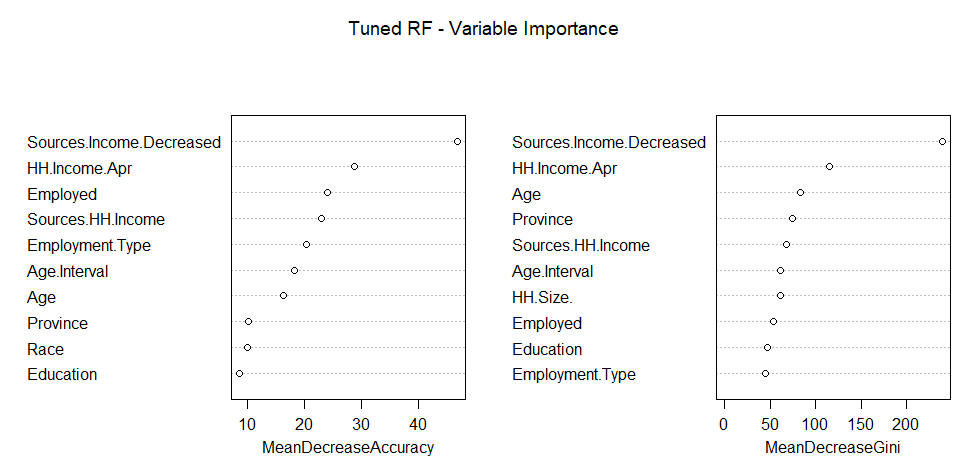
\includegraphics[width=1\linewidth]{Figures/rf3_impplot} \caption{\label{varimprf1} RF Feature Importance}\label{fig:varimprf1}
\end{figure}

\hypertarget{model-2-gbm}{%
\subsection{Model 2: GBM}\label{model-2-gbm}}

The GBM model reports a classification accuracy of 0.70, which is
slightly lower than that achieved by the RF model. In fact, it performs
worse in every metric, except for sensitivity - the number of correct
positive predictions divided by the total number of positives. Figure
\ref{comparison} gives a full overview of the comparison between the two
models, while Figure \ref{gbm_impplot} below reports the feature
importance plot for the GBM.

\begin{figure}[H]
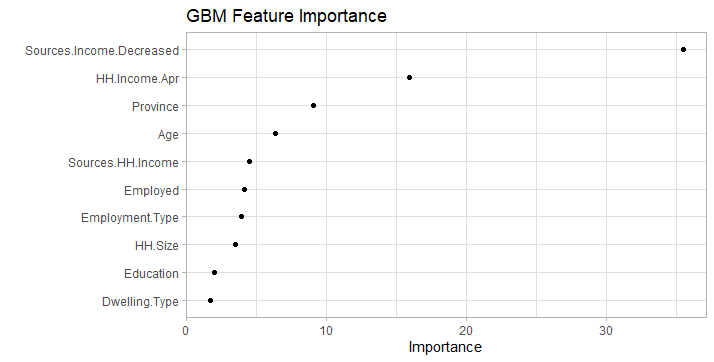
\includegraphics[width=1\linewidth]{Figures/gbm_impplot} \caption{\label{gbm_impplot} GBM Feature Importance}\label{fig:gbm_impplot}
\end{figure}

\hypertarget{comparison}{%
\subsection{Comparison}\label{comparison}}

As seen in Figures \ref{varimprf1} and \ref{gbm_impplot}, both the RF
model and the GBM model largely identify the same 10 features as being
the most important in classifying income change, however, with
differences in ordering. Province and Age seem to be more important in
the GBM model, whilst employment status and type are more crucial in the
RF model. Whether any source of income decreased and total household
income, however, are the most important features throughout. In terms of
classification accuracy, Figure \ref{comparison} below compares the two
models in terms of some of the most important statistics derived from
the respective confusion matrices. It is clear that the RF algorithm
outperforms the GBM algorithm for most metrics, the most important of
which is Accuracy, which gives and indication of the ratio of correct
predictions to total predictions. Likewise, both the RF and GBM models
have low Cohen's kappa values, indicating lower classification
performance in the case of imbalanced data. Lastly, both models are
better at correctly classifying negative cases - specificity (those who
did not lose their main source of income post-lockdown) - compared to
positive cases - sensitivity (those who lost their main source of
income).\footnote{This can be seen in the Appendix \ref{roc} when
  comparing the ROC curves, as well.} Ideally, one would prefer to be
able to more accurately classify the latter group compared to the
former, as it is more useful for policy-makers to protect groups that
are more at risk of losing their main income source.

\begin{figure}[H]
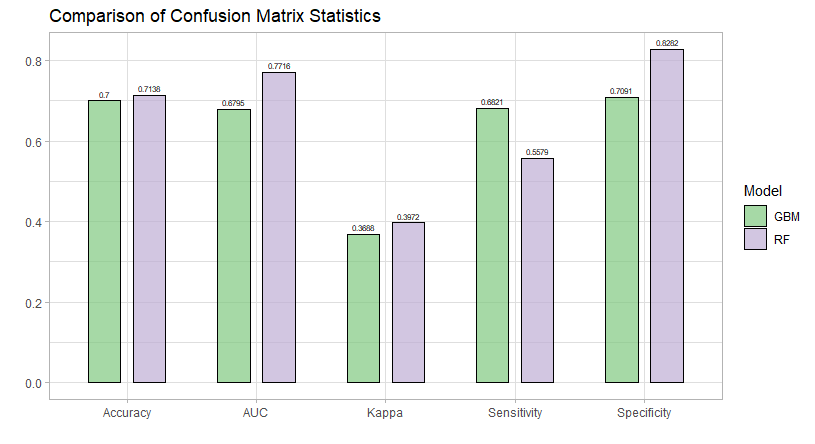
\includegraphics[width=1\linewidth]{Figures/comparison_plot} \caption{\label{comparison} Comparison}\label{fig:comparison}
\end{figure}

Although these results are not ideal, it is clear that they could
perhaps form the baseline for a deeper classification study. For
instance, one could attempt to lower overfitting in the RF model, or
drop some of the features in order to cross-validate results. One could
also train a XGBoost model in order to increase classification
performance, or attempt to repeat this process on a different dataset
with a similar outcome variable. These additions, although not included
in the current report due to time and resource constraints, leave
considerable scope for further model improvements and robustness checks.

\hypertarget{conclusion}{%
\section{Conclusion}\label{conclusion}}

This report attempted to compare two models - a Random Forest and simple
Gradient-Boosted Model - on their performance in classifying which
individuals would lose their main source of income given the South
African Covid-19-induced lockdown. Models were trained on subsamples of
NIDS-CRAM data and tested on testing subsamples, where missing values
were imputed using random forest methods. Model results indicate
relative accuracy, around 70\% for both models. However, the RF
outperforms the GBM in most confusion matrix statistics. Lastly, as
expected, some of the most important features for classification are
household income, employment status and type, province of residence and
age. There remains much scope for additional tuning and model
performance enhancement in the future, as well as the possibility of
additional studies that utilise these methods and data in order to
answer varying classification-type problems. This is especially useful
in the times of Covid-19, where accurate machine learning algorithms
could help address the problematic socioeconomic aspects of lockdown.

\newpage

\hypertarget{references}{%
\section*{References}\label{references}}
\addcontentsline{toc}{section}{References}

\hypertarget{refs}{}
\leavevmode\hypertarget{ref-boehmke}{}%
Boehmke, B. \& Greenwell, B.M. 2019. \emph{Hands-on machine learning
with r}. ed. CRC Press.

\leavevmode\hypertarget{ref-nids2020}{}%
Ingle, K., Brophy, T. \& Daniels, R. 2020. National income dynamics
study--coronavirus rapid mobile survey (nids-cram) panel user manual.
\emph{Technical Note Version}. 1.

\leavevmode\hypertarget{ref-Texevier}{}%
Katzke, N.F. 2017. \emph{Texevier: Package to create elsevier templates
for rmarkdown}. ed. Stellenbosch, South Africa: Bureau for Economic
Research.

\leavevmode\hypertarget{ref-stekhoven2012missforest}{}%
Stekhoven, D.J. \& Bühlmann, P. 2012. MissForest---non-parametric
missing value imputation for mixed-type data. \emph{Bioinformatics}.
28(1):112--118.

\leavevmode\hypertarget{ref-tang2017random}{}%
Tang, F. \& Ishwaran, H. 2017. Random forest missing data algorithms.
\emph{Statistical Analysis and Data Mining: The ASA Data Science
Journal}. 10(6):363--377.

\newpage

\hypertarget{appendix}{%
\section*{\texorpdfstring{Appendix
\label{Appendix}}{Appendix }}\label{appendix}}
\addcontentsline{toc}{section}{Appendix \label{Appendix}}

\hypertarget{rf-plots}{%
\subsection*{\texorpdfstring{RF Plots
\label{rfappendix}}{RF Plots }}\label{rf-plots}}
\addcontentsline{toc}{subsection}{RF Plots \label{rfappendix}}

\begin{figure}[H]

{\centering 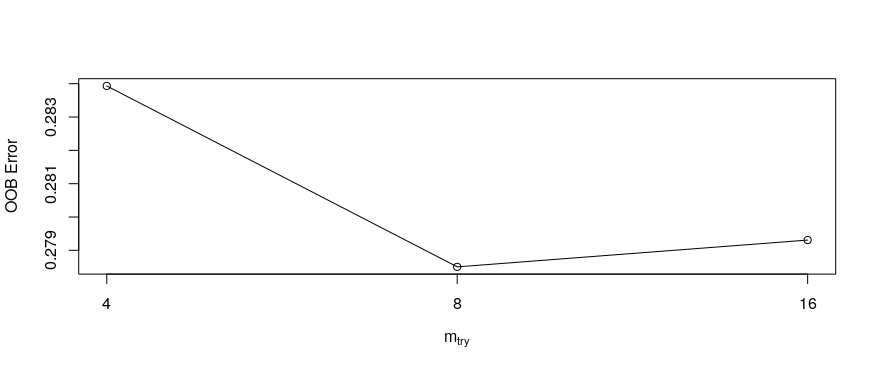
\includegraphics[width=0.8\linewidth,height=0.3\textheight]{Figures/rf1tuned} 

}

\caption{\label{tune} Mtry tuning Plot}\label{fig:tune}
\end{figure}

\begin{figure}[H]

{\centering 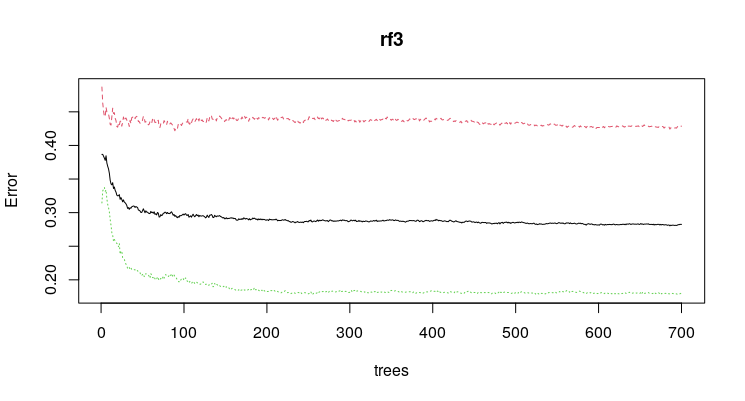
\includegraphics[width=0.8\linewidth,height=0.3\textheight]{Figures/rf3_error_1} 

}

\caption{\label{rferror} Error Plot}\label{fig:rferror}
\end{figure}

\begin{figure}[H]

{\centering 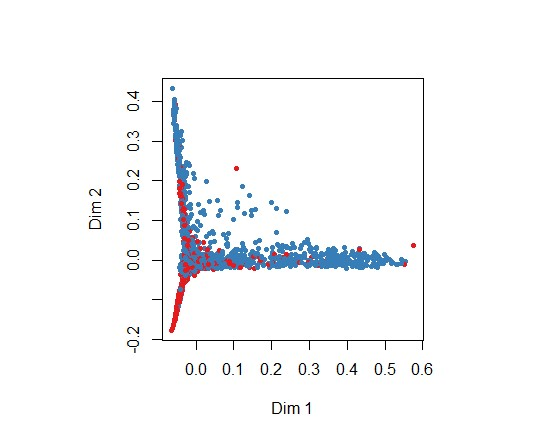
\includegraphics[width=1\linewidth,height=0.35\textheight]{Figures/MDS_rf3_train} 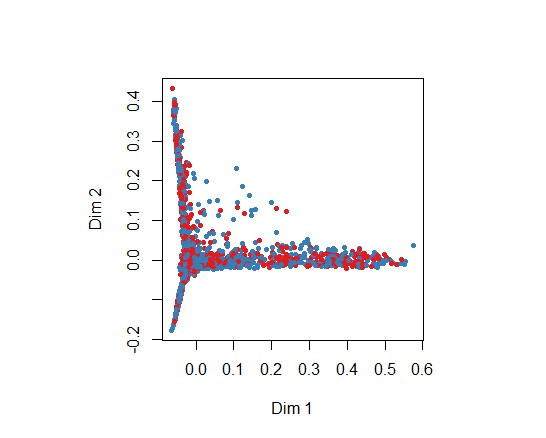
\includegraphics[width=1\linewidth,height=0.35\textheight]{Figures/MDS_rf3_test} 

}

\caption{\label{MDSrf3} Multi-dimensional Scaling plots - Training Data (Top), Test Data (Bottom)}\label{fig:MDSrf3}
\end{figure}

\hypertarget{roc-curves}{%
\subsection*{\texorpdfstring{ROC Curves
\label{roc}}{ROC Curves }}\label{roc-curves}}
\addcontentsline{toc}{subsection}{ROC Curves \label{roc}}

\begin{figure}[H]

{\centering 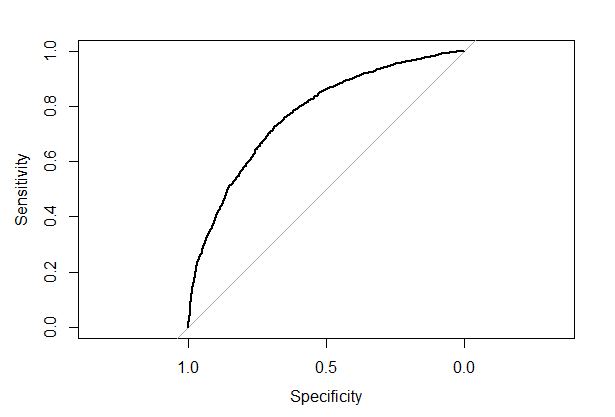
\includegraphics[width=0.49\linewidth,height=0.3\textheight]{Figures/rf3_roc} 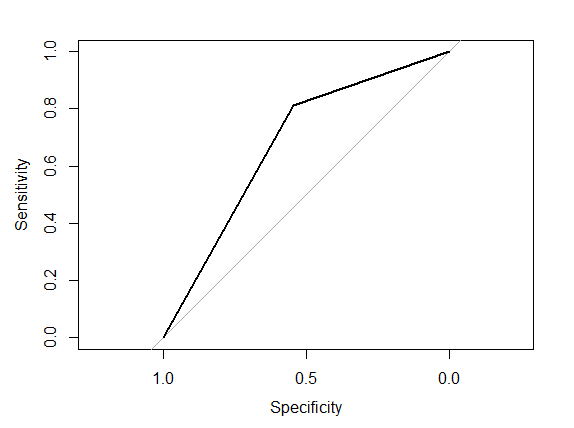
\includegraphics[width=0.49\linewidth,height=0.3\textheight]{Figures/gbm1_roc} 

}

\caption{\label{rf3_roc} ROC curves - RF (left), GBM (right)}\label{fig:rf3_roc}
\end{figure}

\bibliography{Tex/ref}





\end{document}
